\section{Visualization Design Principles for Churn Analysis}

\subsection{Audience and Analytical Questions}
The visualization artifact is designed for analysts and customer-retention
stakeholders. The intended use is not only to report how many customers churned,
but to identify which customer groups are above the baseline churn rate and
which groups should be prioritized for retention actions.

The core analytical questions are:
\begin{enumerate}
  \item What is the overall churn baseline?
  \item Which customer segments are large enough to matter operationally?
  \item Which segments have churn rates above the baseline?
  \item Which features are actionable for a retention team?
  \item How do model outputs support, but not replace, business interpretation?
\end{enumerate}

\subsection{Metric Semantics}
The report separates distribution metrics from risk metrics. This distinction
is essential because a segment can contain many customers but still have an
average churn rate, while a smaller segment can have a much higher churn rate.

\begin{longtable}{p{0.25\textwidth}p{0.35\textwidth}p{0.30\textwidth}}
\caption{Metric definitions used in the visualization design}\\
\toprule
\textbf{Metric} & \textbf{Definition} & \textbf{Interpretation rule} \\
\midrule
\endfirsthead
\toprule
\textbf{Metric} & \textbf{Definition} & \textbf{Interpretation rule} \\
\midrule
\endhead
Customer count &
Number of customers in a segment. &
Measures segment size, not churn risk. \\
Churn count &
Number of churned customers in a segment. &
Useful for workload sizing, but affected by segment size. \\
Churn rate &
Churn count divided by all customers in the same segment. &
Measures within-segment risk and should be compared with the 9.92\% baseline. \\
Share of churned customers &
Churned customers in a segment divided by all churned customers. &
Shows composition of churned customers only; values can sum to 100\%. \\
Predicted churn probability &
Model-estimated probability of churn for customers or groups. &
Useful for prioritization, not as a final business decision by itself. \\
Risk level &
Grouped model or rule-based risk category. &
Should use consistent thresholds and colors across pages. \\
\bottomrule
\end{longtable}

\subsection{Chart Selection by Analytical Task}
The chart type should follow the task, not the visual style preference. The
current churn project mainly contains table data, so the most relevant chart
families are bar charts, distribution charts, relationship views, and summary
tables.

\begin{table}[h]
\centering
\caption{Recommended chart types for churn analysis tasks}
\begin{tabularx}{\textwidth}{p{0.22\textwidth}p{0.30\textwidth}X}
\toprule
\textbf{Task} & \textbf{Recommended chart} & \textbf{Churn example} \\
\midrule
Compare counts & Grouped bar chart & Churn vs. non-churn by satisfaction group \\
Compare risk & Bar chart with baseline & Churn rate by complaint group \\
Show distribution & Histogram or box plot & Credit score or monthly charges \\
Show composition & 100\% stacked bar & Share of churned customers by segment \\
Show relationship & Scatter, heatmap, or small multiples & Satisfaction vs. complaints \\
Show model behavior & Metric cards and confusion matrix & AUC, precision, recall, F1-score \\
\bottomrule
\end{tabularx}
\end{table}

\subsection{Visual Encoding Rules}
The design should use encodings that are easy to decode:
\begin{itemize}
  \item Use position and bar length for comparing counts, churn rates, and
  feature importance.
  \item Use color hue for categorical distinction such as churn versus
  non-churn or low/medium/high risk.
  \item Use a baseline line for churn-rate charts so above-baseline groups can
  be detected quickly.
  \item Avoid pie charts, donut charts, and 3D charts when accurate comparison
  is required.
  \item Avoid using color as the only carrier of meaning; pair color with
  labels, ordering, or reference lines.
\end{itemize}

\subsection{Color System}
The color system should encode meaning consistently. A single default blue for
all charts is visually clean but does not communicate risk hierarchy. The
recommended semantic palette is:

\begin{table}[h]
\centering
\caption{Suggested semantic color palette}
\begin{tabular}{lll}
\toprule
\textbf{Meaning} & \textbf{Color role} & \textbf{Suggested hex} \\
\midrule
Churn / high risk & Highlight and warning & \#D55E00 \\
Medium risk & Intermediate priority & \#E69F00 \\
Low risk & Safer segment & \#009E73 \\
Neutral count / selected bar & Main neutral blue & \#2563EB \\
Not churn / inactive context & Supporting gray-blue & \#64748B \\
Background & Page background & \#F8FAFC \\
Gridline / border & Low-contrast structure & \#E5E7EB \\
\bottomrule
\end{tabular}
\end{table}

These colors should remain stable across pages. For example, high-risk
customers should not be blue on one page and orange on another page. If color is
used to highlight a high-risk segment, the chart should also include a label or
baseline marker so that the message is still readable without color.

\subsection{Page-Level Visualization Structure}
The final visualization artifact can be organized as a compact story rather
than a collection of independent charts:
\begin{enumerate}
  \item \textbf{Overview}: show total customers, churn count, non-churn count,
  baseline churn rate, and risk-level distribution.
  \item \textbf{Churn drivers}: compare feature-group churn rates against the
  baseline and show top model feature importance.
  \item \textbf{Churn-only composition}: show the share of churned customers by
  selected segment, while clearly stating that the denominator is churned
  customers only.
  \item \textbf{Model evaluation}: show AUC, accuracy, precision, recall,
  F1-score, confusion matrix, and a short interpretation of model limitations.
  \item \textbf{Prediction and retention priority}: show predicted churn
  customers, risk levels, and the features that define priority groups.
\end{enumerate}

\subsection{Final Dashboard Screenshots}
The final reporting artifact contains three dashboard pages. The pages do not
implement every recommended technique from the design checklist, but they are
used as the final version for the project report due to time constraints. The
most important requirement is that the interpretation remains clear: KPI cards
summarize the problem size, bar charts compare segment risk, and model outputs
support retention prioritization.

\begin{figure}[p]
\centering
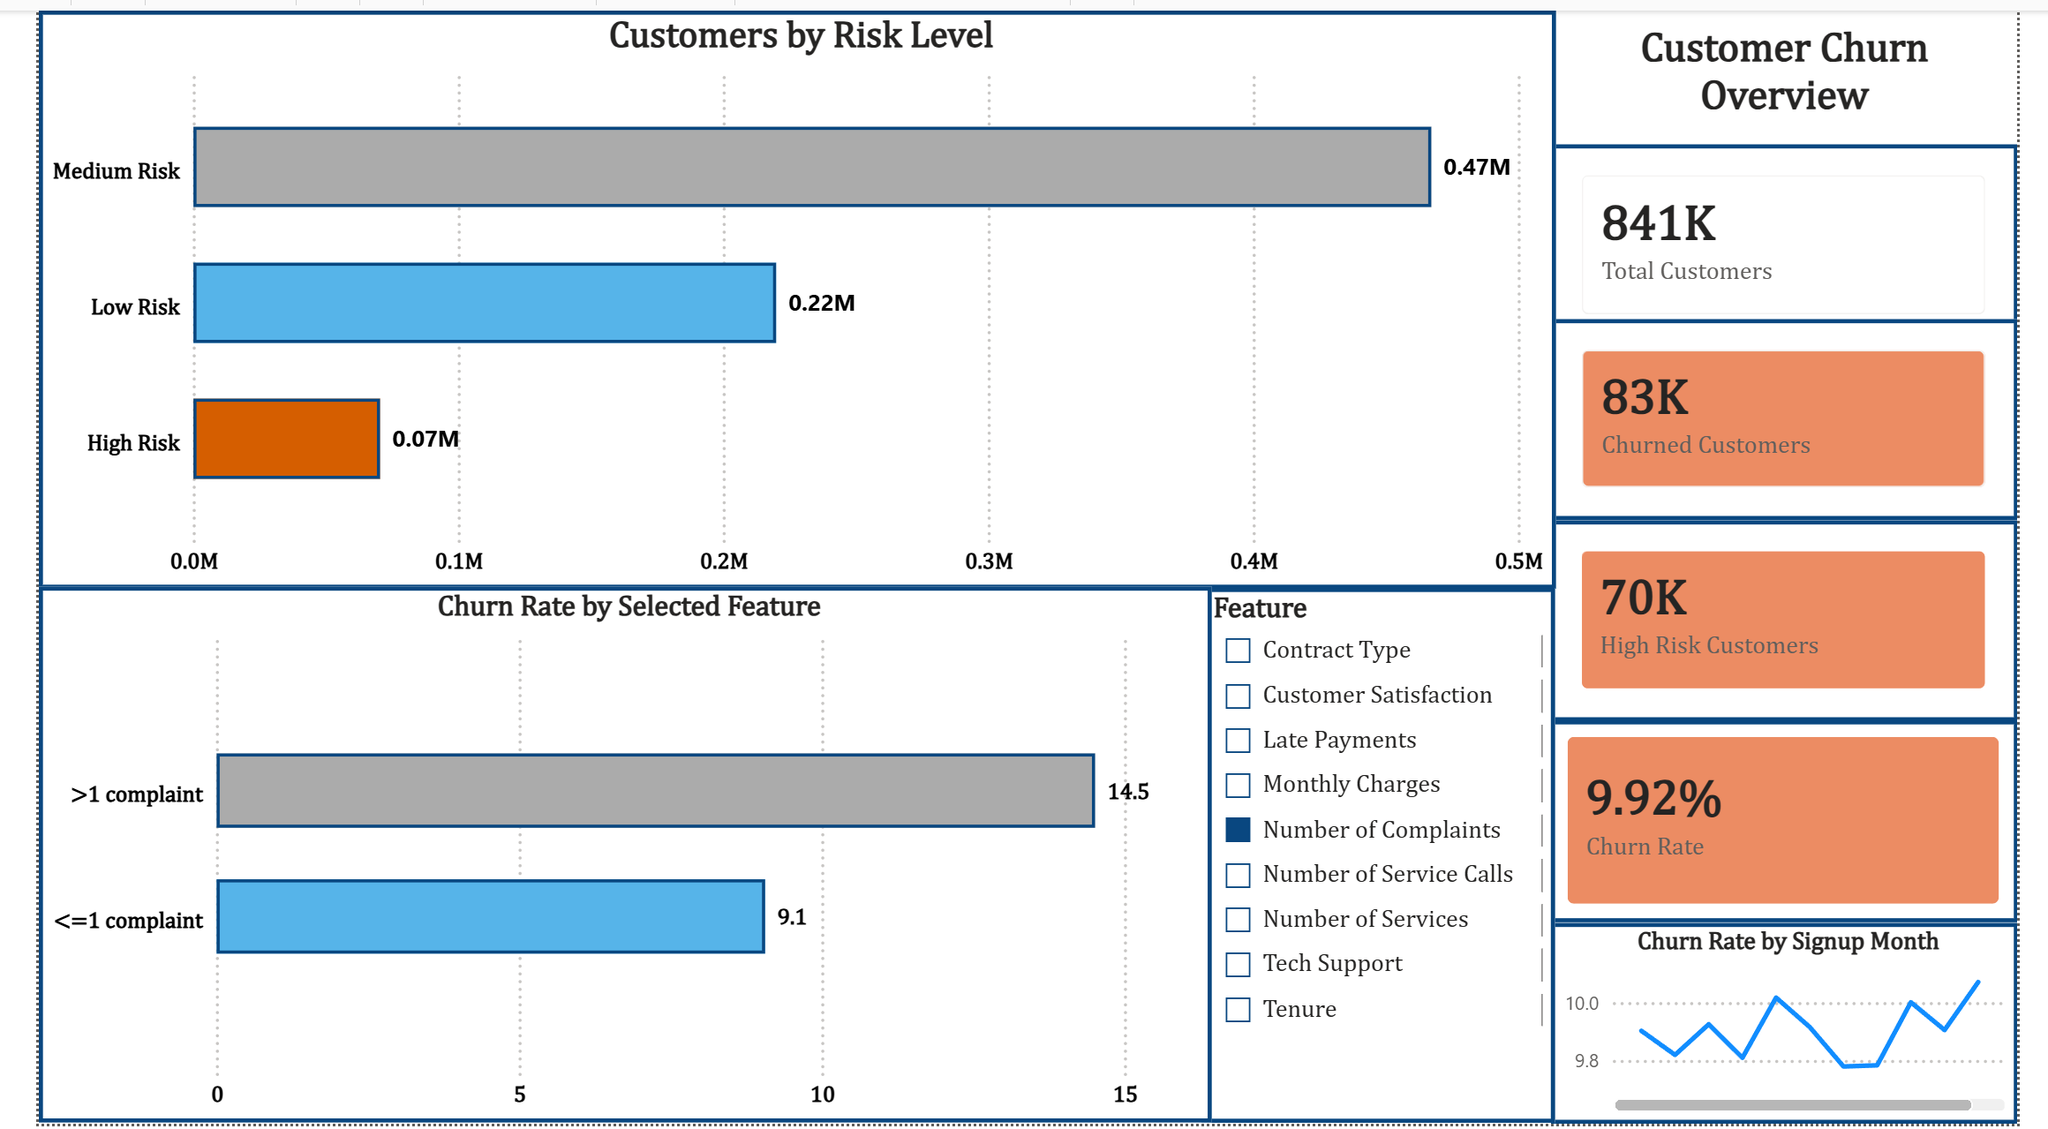
\includegraphics[width=\textwidth]{figures/dashboard_overview.png}
\caption{Final dashboard page 1: customer churn overview, KPI cards, risk-level distribution, selected-feature churn rate, and signup-month trend.}
\label{fig:dashboard_overview}
\end{figure}

\begin{figure}[p]
\centering
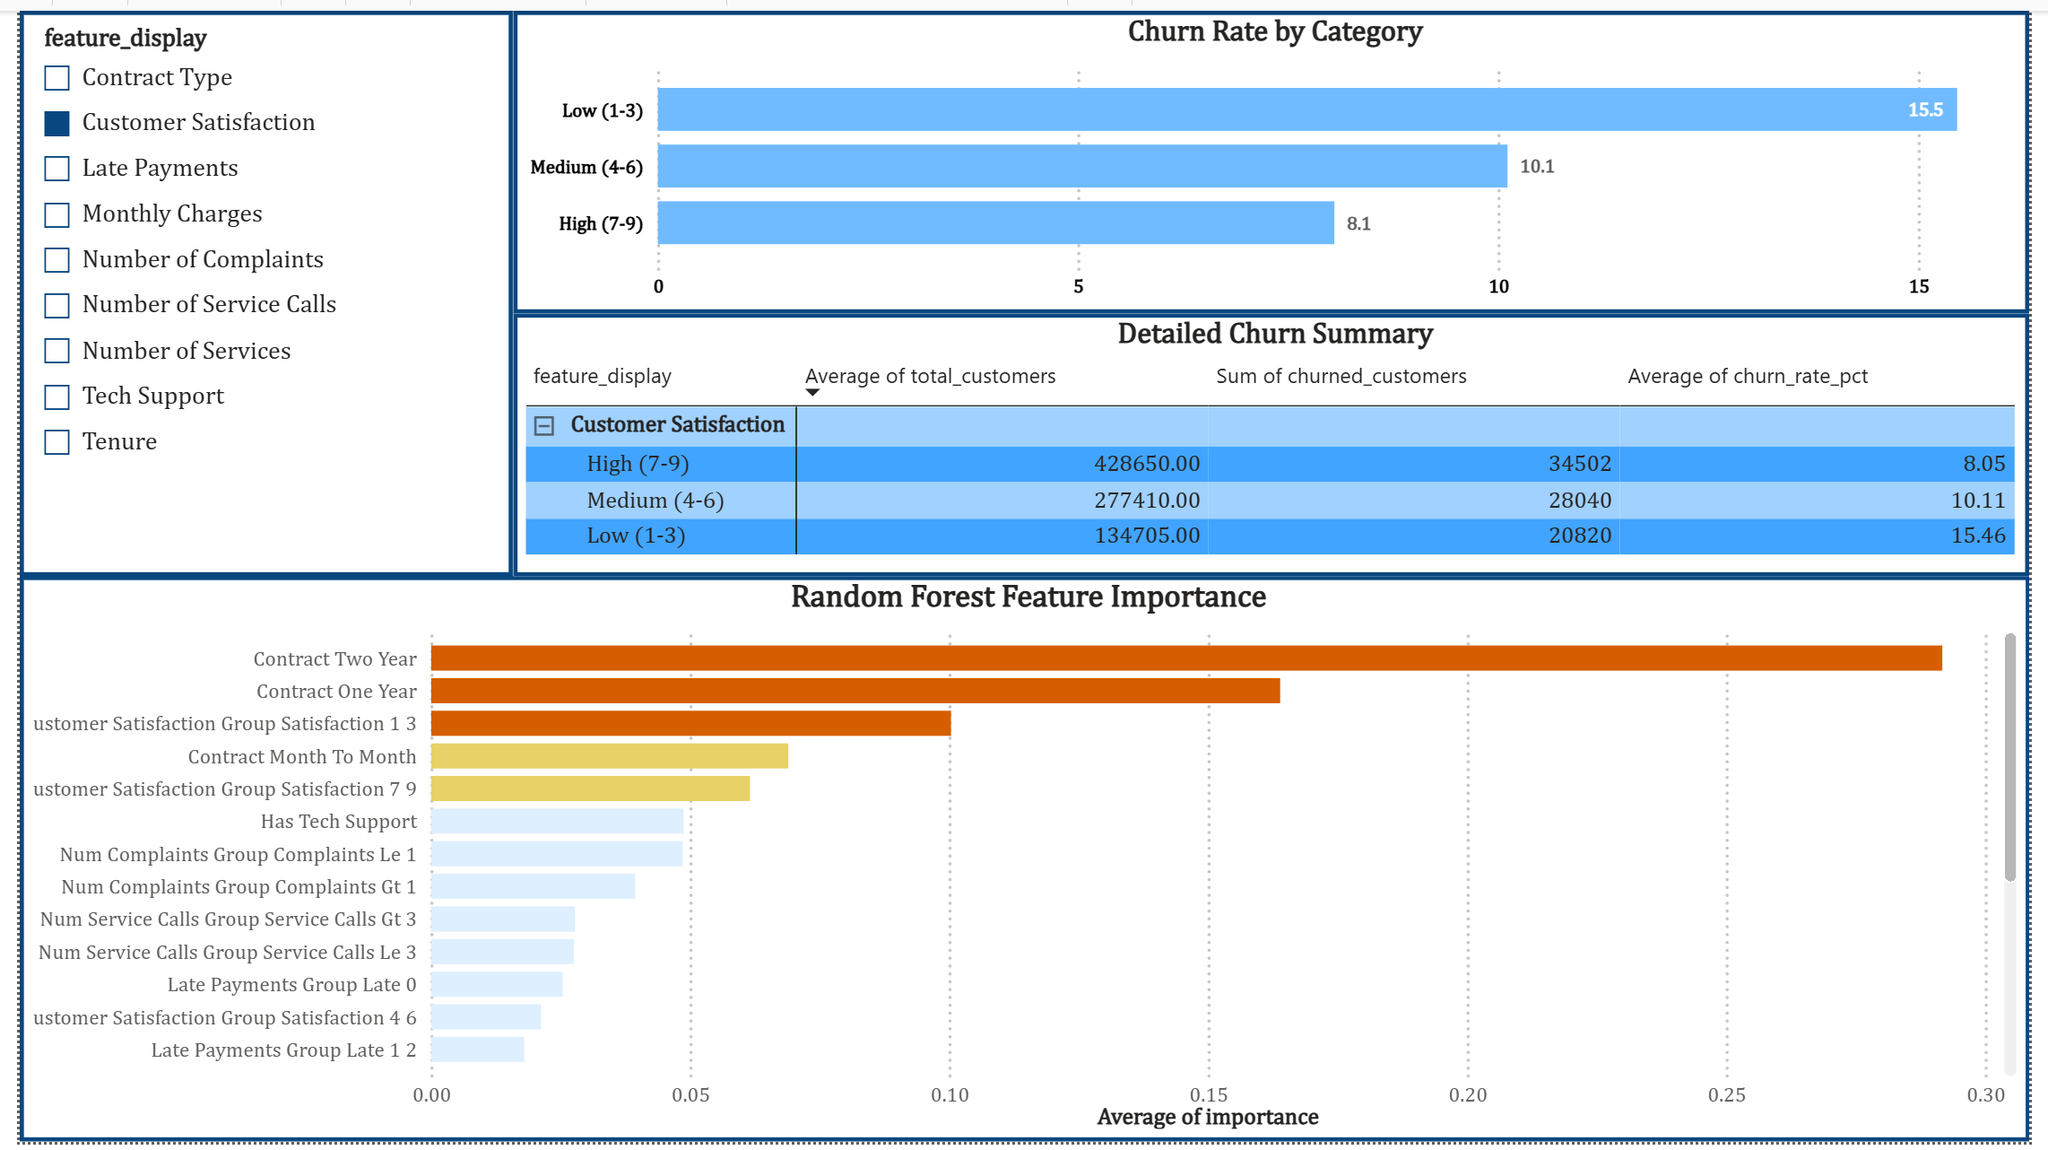
\includegraphics[width=\textwidth]{figures/dashboard_drivers.png}
\caption{Final dashboard page 2: churn driver detail page with feature filter, churn-rate-by-category view, detailed summary table, and Random Forest feature importance.}
\label{fig:dashboard_drivers}
\end{figure}

\begin{figure}[p]
\centering
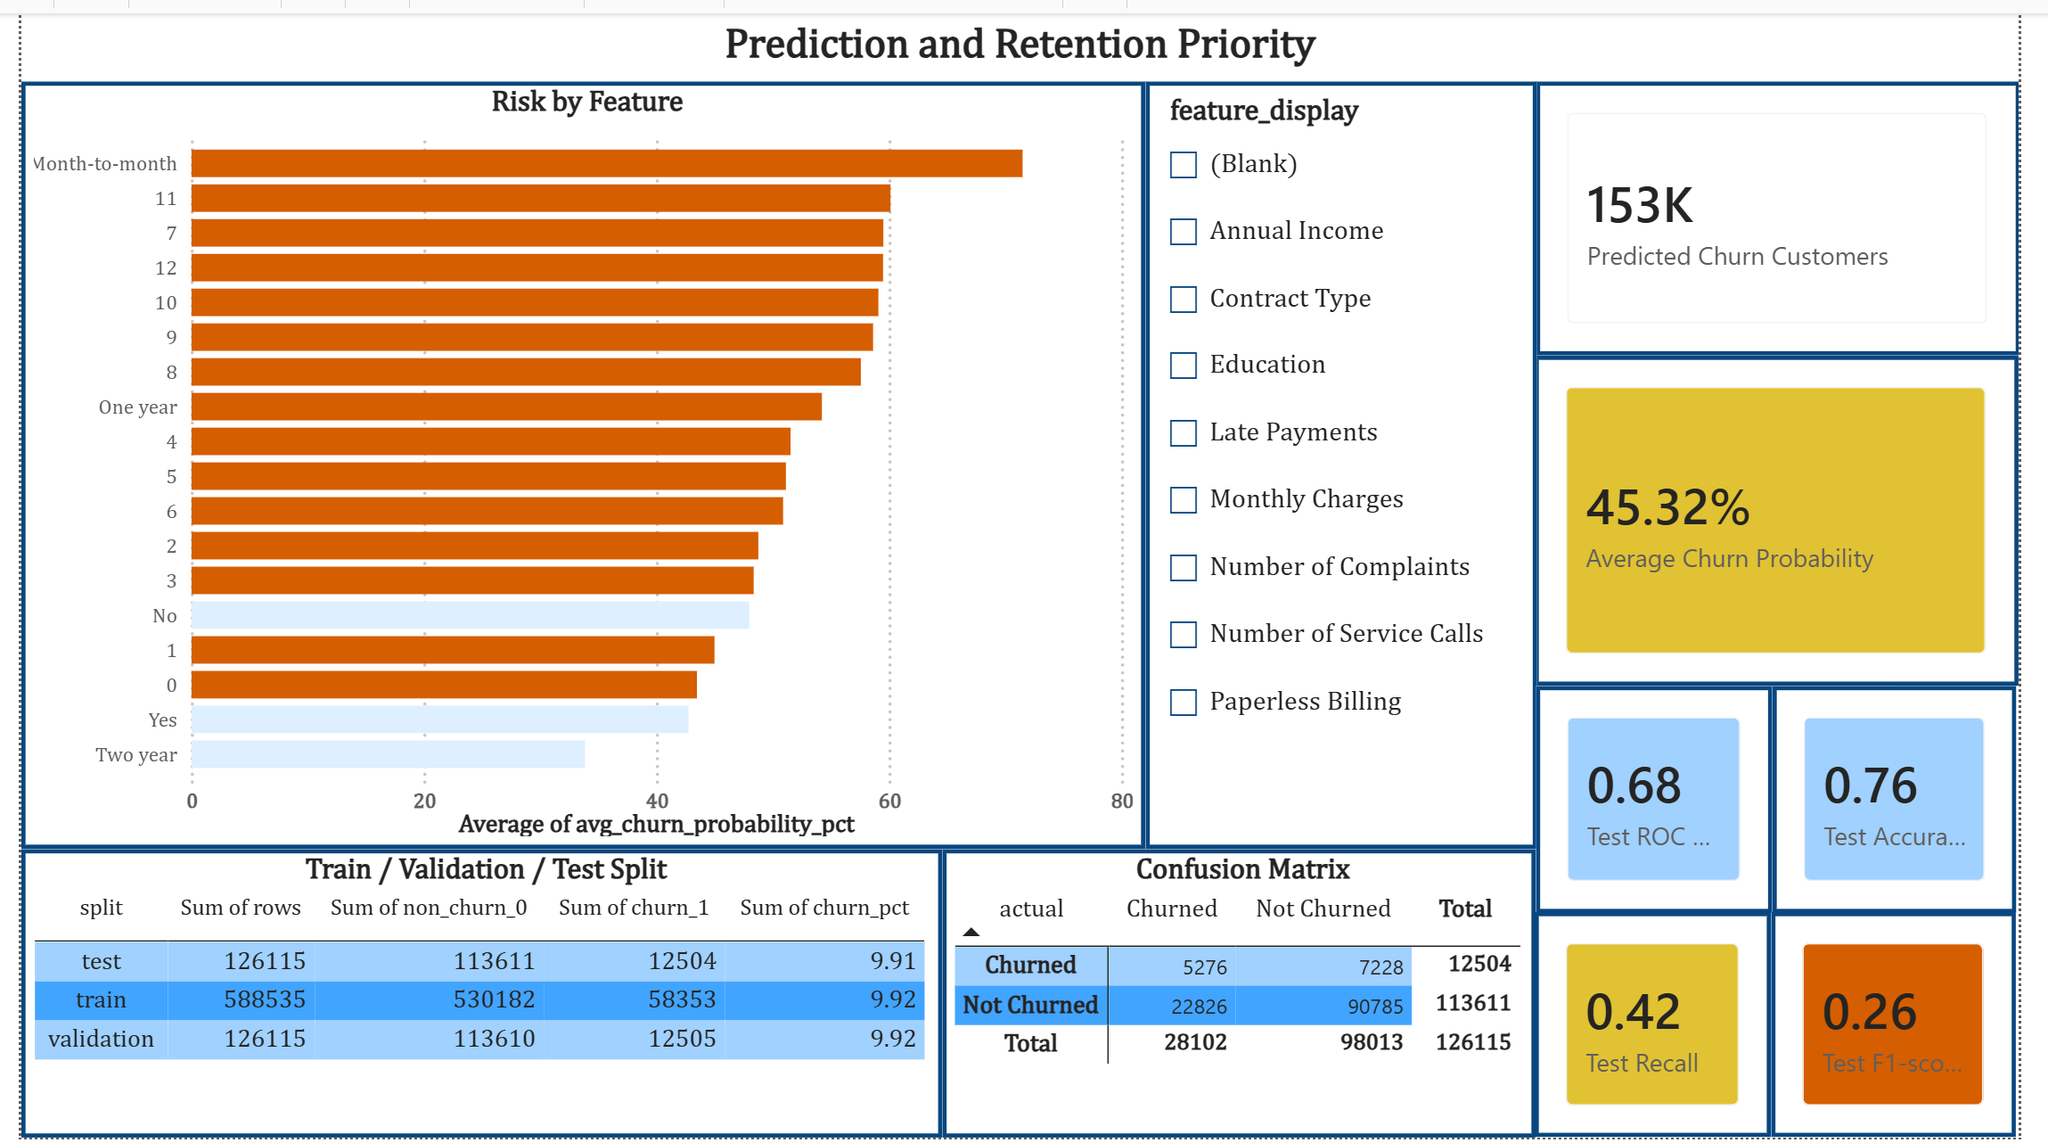
\includegraphics[width=\textwidth]{figures/dashboard_prediction.png}
\caption{Final dashboard page 3: prediction and retention priority page with risk-by-feature view, predicted churn KPIs, train/validation/test split, and confusion matrix.}
\label{fig:dashboard_prediction}
\end{figure}

\subsection{Figure Quality Checklist}
When reading the final screenshots, each chart should be checked against the
following criteria:
\begin{itemize}
  \item The title states either the analytical question or the main insight.
  \item The denominator of every percentage or rate is explicit.
  \item Count views and churn-rate views are not mixed into one ambiguous
  metric.
  \item Churn-rate charts include the 9.92\% baseline reference.
  \item Category order is meaningful: ordinal groups keep natural order, while
  nominal groups are sorted by value only when ranking is intended.
  \item Colors are semantic and consistent across pages.
  \item The chart avoids 3D effects, unnecessary decoration, and hard-to-read
  legends.
\end{itemize}
